\par
L'interface graphique offre la possibilité à l'utilisateur d'interagir avec l'application.

\begin{figure}[!h]
	\centering
   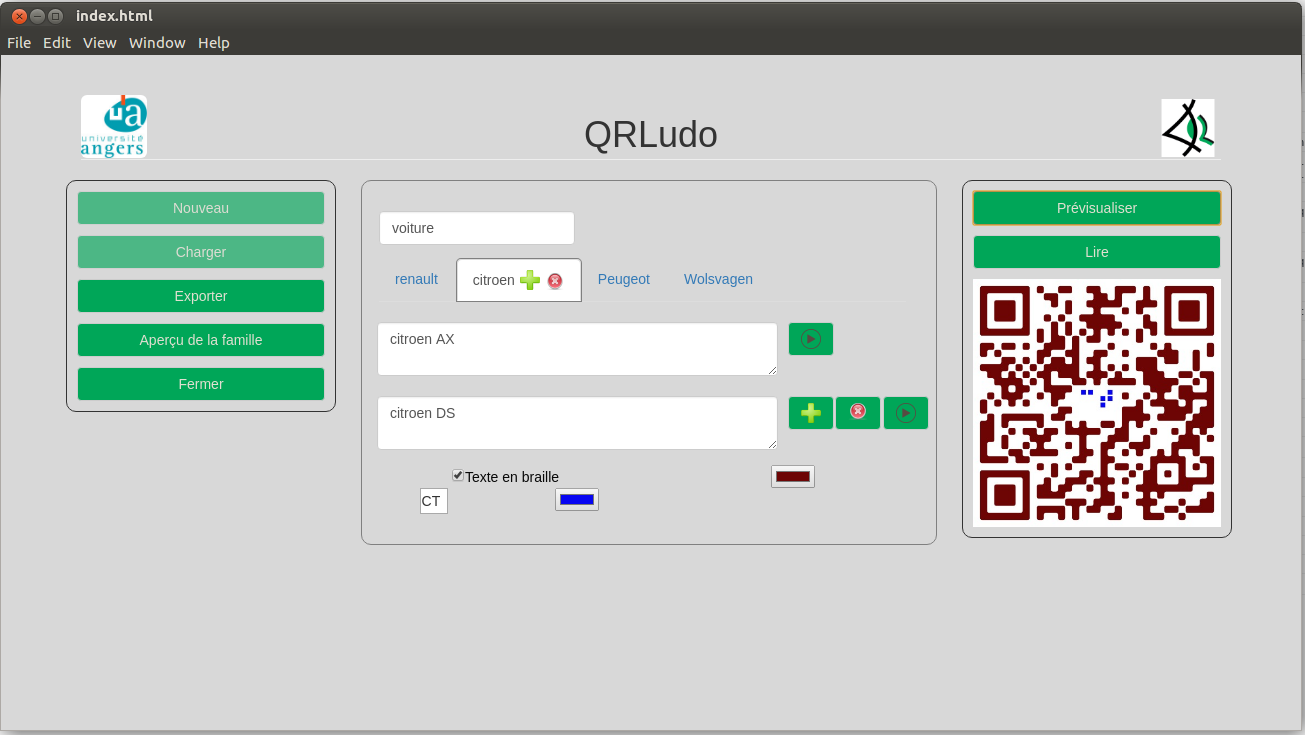
\includegraphics[scale=0.25]{img/interface.png}
   \caption{Interface de création d'une famille de qrcodes}
\end{figure}

\par
Elle est constituée de trois blocs partant de la gauche vers la droite : 
\begin{enumerate}
\item Bloc 1 : partant de haut en bas, il regroupe les boutons permettant les opérations suivantes :
	\begin{itemize}
	\item la création d'un nouveau projet de QR Code unique ou d'une famille de QR Codes.
	\item l'importation d'un projet de QR Code unique ou d'une famille de QR Codes.
	\item l'exportation d'un projet de QR Code unique ou d'une famille de QR Codes.
	\item l'aperçu de l'image d'une famille de QR Codes.

\begin{figure}[!h]
			\centering
		   	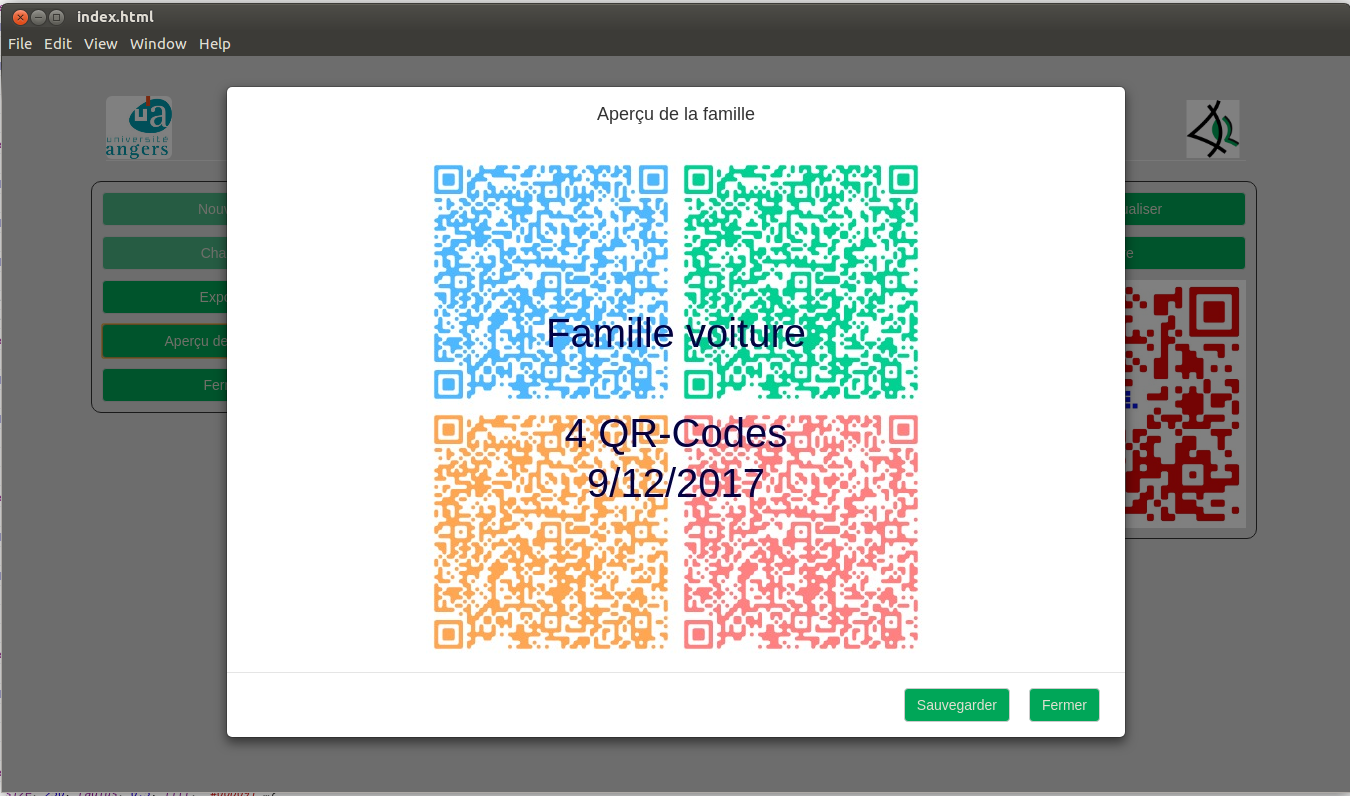
\includegraphics[scale=0.25]{img/image-famille.png}
		   	\caption{Aperçu d'une image famille de QR Codes}
		\end{figure}
	
	Les boutons Sauvegarder et Fermer permettent de sauvegarder le projet et de fermer l'aperçu.\\
	\item la fermeture d'un projet.
	\end{itemize}

\newpage
\item Bloc 2 : il contient un formulaire qui regroupe des champs (musique ou texte). À coté de chaque champ se trouvent des boutons pour créer, supprimer et lire le contenu du champ par synthèse vocale.\\
À la fin du formulaire, de la gauche vers la droite, se trouvent :
	\begin{itemize}
	\item une case à cocher pour afficher ou masquer les options du texte en braille à savoir le texte et la couleur du texte via une palette de couleurs. Notons que le texte en braille ne peut pas dépasser deux caractères, afin de ne pas empêcher la lecture du QR Code.
	\item une palette de couleurs pour la couleur du QR Code.
	\end{itemize}
Dans le cas d'un projet de famille de QR Codes, on note l'apparition :
	\begin{itemize}
	\item d'une zone de texte pour le nom de la famille, en haut du formulaire.
	\item d'une liste d'onglets, chacun faisant référence à un formulaire. À coté de chaque onglet, figurent deux boutons pour ajouter un onglet ou supprimer l'onglet actif; chaque onglet représente un QR Code.
	\end{itemize}
	
\item Bloc 3 : partant du haut vers le bas, il contient : 
	\begin{itemize}
	\item un bouton pour prévisualiser un QR Code à partir des informations du formulaire (celui de l'onglet actif dans le cas d'un projet de famille de QR Codes).
	\item un bouton lire pour lire par synthèse vocale tous les champs du formulaire (le formulaire de l'onglet actif dans le cas d'une famille de QR codes).
	\end{itemize}

\end{enumerate}

\par
Un manuel plus exhaustif destiné aux utilisateurs de l'application est disponible en annexe de ce dossier (\ref{manuel}).

